\section{Density estimation}

For calculating the probability of a logical expression, we can employ the following summation formula:
\[\textnormal{P}(E)=\sum_{row \backsim E}\textnormal{P}(row)\]
To compute inference, we can use the formula:
\[\textnormal{P}(E_1|E_2)=\dfrac{\textnormal{P}(E_1 \land E_2)}{E_2}=\dfrac{\sum_{row \backsim E_1 \land E_2}\textnormal{P}(row)}{\sum_{row \backsim E_2}\textnormal{P}(row)}\]
\begin{example}
    Given the following truth table: 
    \begin{table}[H]
        \centering
        \begin{tabular}{ccc|c}
        \hline
        $\boldsymbol{A}$ & $\boldsymbol{B}$ & $\boldsymbol{C}$ & $\boldsymbol{\textnormal{\textbf{P}}(A,B,C)}$ \\ \hline
        0   & 0   & 0   & 0.30       \\ 
        0   & 0   & 1   & 0.05       \\ 
        0   & 1   & 0   & 0.10       \\ 
        0   & 1   & 1   & 0.05       \\ 
        1   & 0   & 0   & 0.05       \\ 
        1   & 0   & 1   & 0.10       \\ 
        1   & 1   & 0   & 0.25       \\ 
        1   & 1   & 1   & 0.10       \\ \hline
        \end{tabular}
    \end{table}
    $\textnormal{P}(A)$ can be found by summing all the probability where $A=1$, that is: 
    \[\textnormal{P}(A) = 0.05 + 0.10 + 0.25 + 0.10 = 0.5\]
    $\textnormal{P}(A \land B)$ can be found by summing all the probability where $A=1$ and $B=1$, that is: 
    \[P(A \land B) = 0.25 + 0.10 = 0.35\]
    $\textnormal{P}(\overline{A} \lor B)$ can be found by summing all the probability where $A=0$ or $B=1$, that is: 
    \[\textnormal{P}(\overline{A} \lor B) = 0.30 + 0.05 + 0.10 + 0.05 + 0.25 + 0.10 = 0.85\]
    $P(A | B)$ can be found by dividing the probability of $A=1$ and $B=1$ by the probability where $B=1$, that is: 
    \[\textnormal{P}(A | B) = \dfrac{(0.25+0.10)}{(0.10+0.05+0.25+0.10)}=0.7\]
    $\textnormal{P}(C | A \land B)$ can be found by dividing the probability of $A=1$ and $B=1$ and $C=1$ by the probability where $A=1$ and $B=1$, that is: 
    \[\textnormal{P}(C | A \land B) = \dfrac{(0.10)}{(0.25+0.10)}=0.285\]
    $\textnormal{P}(\overline{A} | C)$ can be found by dividing the probability of $A=0$ and $C=1$ by the probability where $C=1$, that is: 
    \[\textnormal{P}(\overline{A} | C) = \dfrac{(0.05+0.05)}{(0.05+0.05+0.10+0.10)}=0.333\]
\end{example}
\begin{definition}[\textit{Density estimator}]
    A density estimator is designed to acquire knowledge in the form of a mapping from a set of attributes to a probability distribution within the attribute space, defined as:
    \[M:\{0,1\}^I \rightarrow [0,1]\]
\end{definition}

\paragraph*{Likelihood density estimators}
We can employ likelihood to assess density estimation. 
When presented with a record $x$, a density estimator $M$ provides an estimate of how probable it is, denoted as $\widehat{\textnormal{P}}(x|M)$. 
When dealing with a dataset containing $N$ records, a density estimator can inform us about the likelihood of the data, assuming that all records were generated independently from it:
\[\widehat{\textnormal{P}}(\textnormal{dataset})=\widehat{\textnormal{P}}(x_1,x_2,\dots,x_N)=\prod_{n=1}^{N}\widehat{\textnormal{P}}(x|M)\]
Due to the potential issue of likelihood values becoming extremely small, it's common practice to work with log-likelihood instead:
\[\log{\widehat{\textnormal{P}}(\textnormal{dataset})}=\log{\prod_{n=1}^{N}{\widehat{\textnormal{P}}(x_n|M)}}=\sum_{n=1}^{N}{\log{\widehat{\textnormal{P}}(x_n|M)}}\]

Density estimators offer a range of valuable capabilities, including the ability to order records by their probability, which can help identify outliers or anomalies. 
They are also instrumental in inference tasks and can serve as a foundation for Bayes classifiers. 
However, it's important to note that the primary challenge with joint density estimators is their susceptibility to severe overfitting.

\paragraph*{Naïve density estimators}
The naïve Bayes estimator model operates under the assumption that each attribute is independent of the others. 
Using the notation where $x[i]$ represents the $i^{th}$ field of record $x$ the naïve density estimator posits that:
\[x[i] \perp \{x[1],x[2],\dots,x[i-1],x[i],x[i+1],\dots,x[I]\}\]
It's crucial to acknowledge that in the naïve Bayes estimator model, all attributes are treated as equally important, and the model assumes that the knowledge of one attribute conveys no information about the value of another. 
While this final assumption is rarely accurate in real-world scenarios, it often yields effective results when applied in practice.
\begin{example}
    In the context of the naïve Bayes estimator model, given four variables $A,B,C$, and $D$, they are all considered independent due to the model's assumptions. Consequently, this implies that:
    \[\textnormal{P}(A,\overline{B},C,\overline{D}) = \textnormal{P}(A)\textnormal{P}(\overline{B})P(C)\textnormal{P}(\overline{D})\]
\end{example}

In order to train a naïve Bayes estimator, we must make the assumption that $x[1],\dots,x[n]$ are independently distributed. 
Under this hypothesis, it becomes feasible to construct any row of the resulting joint distribution as needed:
\[\widehat{\textnormal{P}}(x[1]=u_1,x[2]=u_2,\dots,x[I]=u_I) = \prod_{k=1}^{I} \widehat{\textnormal{P}}(x[k]=u_k)\]
\begin{table}[H]
    \centering
    \begin{tabular}{c|c|c|}
    \cline{2-3}
                                                & \textbf{Joint estimator} & \textbf{Naïve estimator} \\ \hline
    \multicolumn{1}{|c|}{\textbf{Modelling}}   & Anything                 & Boring distributions     \\ 
    \multicolumn{1}{|c|}{\textbf{Attributes}}  & Few Boolean              & Many multivalued         \\ 
    \multicolumn{1}{|c|}{\textbf{Overfitting}} & Yes                      & Quite robust             \\ \hline
    \end{tabular}
\end{table}
\begin{figure}[H]
    \centering
    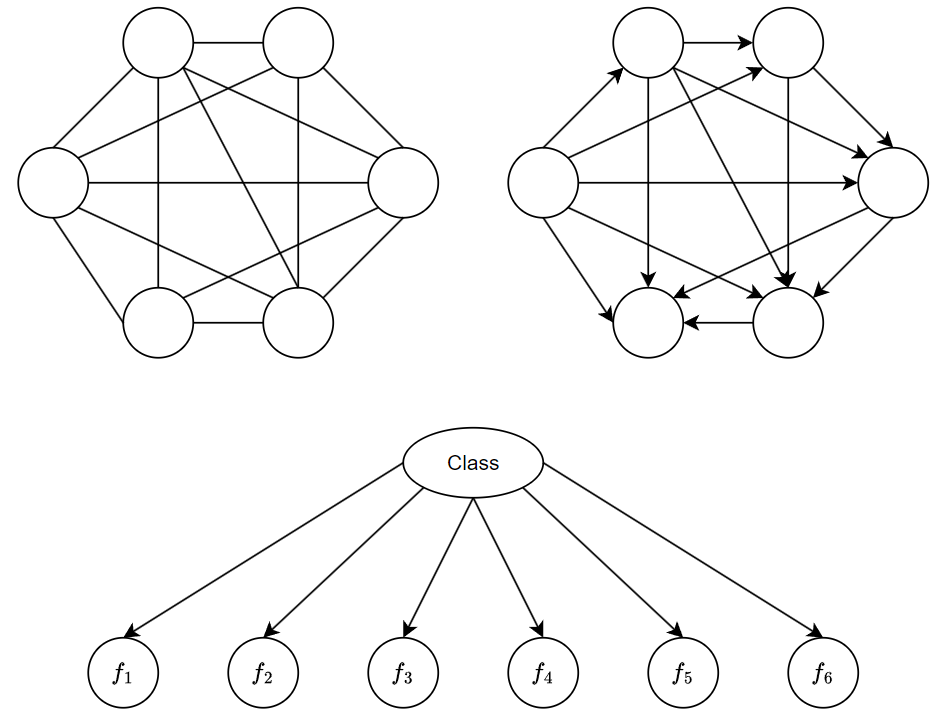
\includegraphics[width=0.5\linewidth]{images/naive-joint.png}
    \caption{Comparison between a joint and a naïve estimator}
\end{figure}